\chapter{Grundlagen}\label{kap:grundlagen}

%####################  CHAPTER 1: Grundlagen  #################

In diesem Kapitel werden zunächst die Grundlagen 
des Machine Learnings mit künstlichen Neuronalen Netzen 
beschrieben. Im zweiten Abschnit werden die sogenannten 
\textit{Convolutional Neural Networks} für die 
Bilderkennung genauer betrachtet.
Der letzte Abschnitt wird die verwendete Hardware,
den \textit{Neural Compute Stick 2} behandeln.


%------------------- SECTION: Machine Learning ------------------

\section{Machine Learning}\label{sec:ml}

Beim Machine Lerining, welches ein Teilgebiet der Computerwissenschafen
ist, geht es um die Erstellung von Algorithmen, die Zusammenhänge in 
großen Datenmengen erkennen können, ohne explizit darauf programmiert
worden zu sein.
Eine Form davon ist das \textit{Supervised Learning}, bei dem das Programm 
neben den Input Daten auch die Zugehörigen Ausgaben, in vorm von 
Labels, erhält um daraus 
Regeln für die Zusammenhänge zwischen Ein- und Ausgabe Daten abzuleiten.
Dadurch unterscheidet sich das Vorgehen, wie in Abbildung 
\ref{fig:ml_classic_programm} veranschaulicht, wesentlich zur klassischen 
Programmierung, bei bei der die Regeln vorab definiert werden müssen.

\vspace{1cm}
\begin{figure}[H]
    \centering
    
\tikzset{
    decision/.style={
        diamond,
        draw,
        text width=4em,
        text badly centered,
        inner sep=-1pt,
        node distance=8em
    },
    block/.style={
        rectangle,
        draw,
        text width=6em,
        %minimum widhth=6em,
        minimum height=3.5em,
        text centered,
        node distance=20em
    },
    arrow/.style={
        draw,
        >=latex,
        ->
    },
    textfeld/.style={
        %draw,
        text centered,
        node distance=1.5em
    }
}


\begin{tikzpicture}

    
    \node (system) [block] {Klassisches\\Programm};
    \node (system2) [block, right of=system] {ML\\Programm};

    \node [textfeld, left=of system.167] (inputs) {Daten};
    \node [textfeld, left=of system.193] (regeln) {Regeln};
    \node [textfeld, right=of system] (output) {Ausgaben};

    \node [textfeld, left=of system2.167] (inputs2) {Daten};
    \node [textfeld, left=of system2.193] (output2) {Ausgaben};
    \node [textfeld, right=of system2] (regeln2) {Regeln};
    
    \draw[arrow] (inputs) -- (system.167);
    \draw[arrow] (regeln) -- (system.193);
    \draw[arrow] (system) -- (output);
    
    \draw[arrow] (inputs2) -- (system2.167);
    \draw[arrow] (output2) -- (system2.193);
    \draw[arrow] (system2) -- (regeln2);
    

\end{tikzpicture}

    \caption{}
    \label{fig:ml_classic_programm}
\end{figure}
\vspace{1cm}


Das ableiten der Regeln erfolgt beim Machine Learning in einem 
iterativen Prozess, welcher als Training bezeichnet wird.
Dabei werden die Zusammenhänge zwischen In- und Output Daten 
als mathematische Funktion betrachtet, welche numerisch 
angenähert wird.

Bei einem linearen Zusammenhang, handelt es sich
um ein Regressions- und bei einem kategorischen um 
eine Klassifikationsproblem.

Weitere Formen neben dem \textit{Supervised Learning} sind das 
\textit{Unsupervised Learning}, bei dem das Programm keine Labels 
erhält, sondern diese selber finden 
soll, oder das \textit{Reinfocement Learning}, bei dem das Programm 
durch interaktion mit der Umwelt bestimmte Aufgaben lernt.
Diese techniken wurden in der Bachelor Arbeit nicht verwendet 
und werden daher nicht näher erläutert.


%------------------- SECTION: Neuronale Netze -------------------

\newpage
\subsection{Künstliche Neuronale Netze} \label{subsec:nn}

Für komplexe Input Daten, wie beispielsweise Bilder, bei denen 
die einzelnen Pixelwerte als Inputs und der Inhalt des Bildes als 
Output dienen, werden in der Regel künstliche Neuronale Netze verwendet.
Diese sind eine Form des Machine Learings und bestehen aus einer 
vielzahl an miteinander verbundener Neuronen. Durch unterschiedlich 
starke Gewichtungen der einzelnen Verbindungen, auch Gewichte genannt, 
können für unterschiedliche Input Daten die entsprechenden Outputs 
gefunden werden.

\vspace{1cm}
\begin{figure}[H]
    \centering
    \label{fig:nn}
    \def\svgwidth{0.85\columnwidth}
    \footnotesize
    \begin{neuralnetwork}[height=1]
    \newcommand{\nodetextclear}[2]{}
    \newcommand{\nodetexth}[2]{$h_#2$}
    \newcommand{\nodetextx}[2]{$x_#2$}
    \newcommand{\nodetexty}[2]{$y_#2$}
    \inputlayer[count=3, bias=false, title=Input\\layer, text=\nodetextx]
    \hiddenlayer[count=4, bias=false, title=Hidden\\layer, text=\nodetexth] \linklayers
    \outputlayer[count=2, title=Output\\layer, text=\nodetexty] \linklayers
\end{neuralnetwork}
\end{figure}
\vspace{1cm}

Die richtige Gewichtung der Parameter erfolgt dabei in dem iterativen
Trainingsprozess, welcher aus den drei schritten:


\begin{itemize}
    \item \textit{Forward Pass} anhand aktueller Gewichte vorhersage aus den Inputs treffen
    \item \textit{Fehlerbestimmung} Abweichung zum tatsächlichen werten berechnen
    \item \textit{Backpropagation} Minimierung des Fehlers durch Anpassung der Gewichte
\end{itemize}

besthet und in Abbildung \ref{fig:train} schematisch dargestellt ist.


\vspace{1cm}
\begin{figure}[H]
    \centering
    
\tikzstyle{process} = [rectangle, fill=blue!20, minimum width=2.5cm, minimum height=1cm, text centered, draw=black]
\tikzstyle{arrow} = [thick,->,>=stealth]

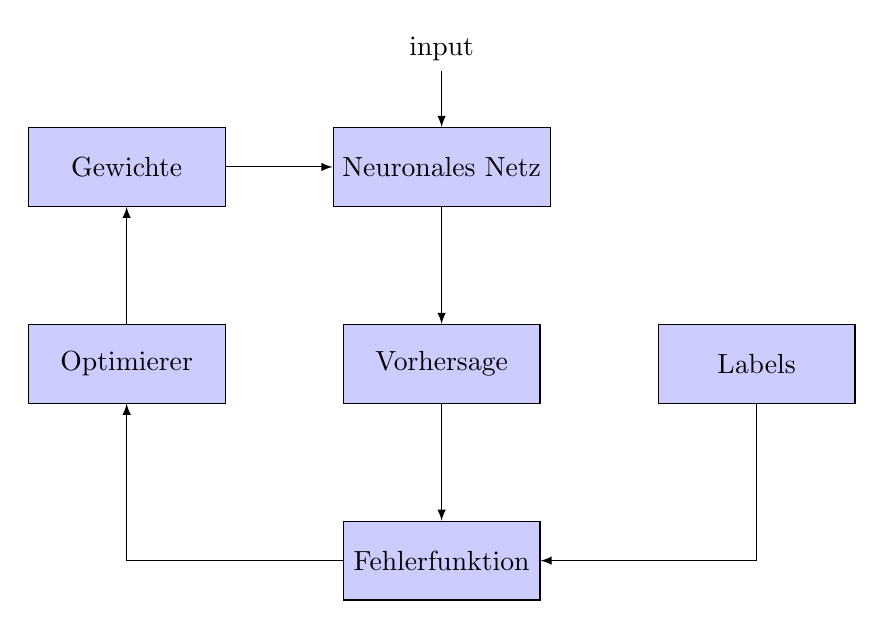
\begin{tikzpicture}[node distance=1.6cm]

  \begin{scope}[node distance=2.5cm]
    \node (nn)      [process]                   {Neuronales Netz};
    \node (pred)      [process, below of=nn]      {Vorhersage};
    \node (loss)      [process, below of=pred]      {Fehlerfunktion};
    
  \end{scope}
  
  \begin{scope}[node distance=4cm]
    \node (opt) [process, left of=pred]      {Optimierer};
    \node (weights)  [process, left of=nn] {Gewichte};
    \node (labels)   [process, right of=pred]  {Labels};
  \end{scope}

  \node (input) at (0,1.5) {input};

  \draw[arrow] (input) -- (nn);

  \draw[arrow] (nn) -- (pred);
  \draw[arrow] (pred) -- (loss);

  \draw[arrow] (labels) |- (loss);
  \draw[arrow] (loss) -| (opt);

  \draw[arrow] (opt) -- (weights);
  \draw[arrow] (weights) -- (nn);
  
    
\end{tikzpicture}

    \caption{Trainingsablauf eines Neuronalen Netzes}
    \label{fig:train}
\end{figure}
\vspace{1cm}




Durch merhfaches durchlaufen dieser Schritte, 
kann die Fehlerfunktion soweit minimiert werden, dass 
das Modell auch für neue, ungesehene Input Daten 
die richtigen Ausgaben vorhersagen kann.
Die Funktionsweisen der einzelnen Schritte 
werden im folgenden näher erläutert.


\subsubsection{Forward Pass}
Im \textit{Forward Pass} werden die Inputs, welche an der 
ersten Schicht aus Neuronen anliegen, durch alle Schichten hindurch 
gereicht, um in der Ausgabeschicht Schicht
das gesuchte Ergebnis zu liefern.
Dabei erhält jedes Neuron die mit dem Parameter $w_{i}$ gewichteten
Ausgabewerte aller Neuronen der vorherigen Schicht und summiert diese
zusammen mit einem konstanten Bias Wert $b$ auf.

Mithilfe einer Aktivierungsfunktion wird der Wert auf
einen bestimmten Bereich skaliert.

Abbildung \ref{fig:neuron} zeigt den Vorgang an einem einzenen 
Neuron.

\vspace{1cm}
\begin{figure}[H]
    \centering
    \begin{tikzpicture}[
    % define styles    
    init/.style={ 
         draw, 
         circle, 
         inner sep=2pt,
         font=\Huge,
         join = by -latex
    },
    squa_draw/.style={ 
        draw,
        font=\Large,
        join = by -latex
    },
    squa/.style={ 
        font=\Large,
        join = by -latex
    }
]
% Top chain x1 to w1
\begin{scope}[start chain=1]
    \node[on chain=1] at (0,1.5cm)  (x1) {$x_1$};
    \node[on chain=1,join=by o-latex] (w1) {$w_1$};
\end{scope}
% Middle chain x2 to output
\begin{scope}[start chain=2]
    \node[on chain=2] (x2) {$x_2$};
    \node[on chain=2,join=by o-latex] {$w_2$};
    \node[on chain=2,init] (sigma) {$\displaystyle\Sigma$};
    \node[on chain=2,squa_draw,label=below:{\parbox{2cm}{\centering Aktivierungs-funktion}}]   {$g(z)$};
    \node[on chain=2,squa,label=below:Output,join=by -latex] {$y_{out}$};
\end{scope}
% Bottom chain x3 to w3
\begin{scope}[start chain=3]
    \node[on chain=3,label=below:Inputs] at (0,-1.5cm) 
    (x3) {$x_3$};
    \node[on chain=3,label=below:Gewichte,join=by o-latex]
    (w3) {$w_3$};
\end{scope}
% Bias
\node[label=above:\parbox{2cm}{\centering Bias \\ $b$}] at (sigma|-w1) (b) {};
% Arrows joining w1, w3 and b to sigma
\draw[-latex] (w1) -- (sigma);
\draw[-latex] (w3) -- (sigma);
\draw[o-latex] (b) -- (sigma);

\end{tikzpicture}

% von https://medium.com/momenton/typesetting-neural-network-diagrams-with-tex-4920b6b9fc19
    \caption{Berechnungen an einem einzelnen Neuron}
    \label{fig:neuron}
\end{figure}
\vspace{1cm}

Um den \textit{Forward Pass} für eine gesammte Schicht, bestehend aus 
einer Vielzahl an Neuronen, zu berechnen, werden die Schichten 
als Vektoren und die Gewichte als Matrizen dargestellt.

Die Matrixmultiplikation aus dem Vektor der vorherigen 
Schicht $x$ mit der Gecwichtsmatrix $W$ ergibt die Werte
des Vektors $z$ der aktuellen Schicht, wie Gleichung 
\ref{eq:forward} zeigt.

\begin{equation}
    \label{eq:forward}
    z = W^{T}x+b
\end{equation}


Dieser Vektor wird dann elementweise einer nichtlinearen
Aktivierungsfunktion $g(z)$ übergeben.

Für mittlere Schichten (\textit{Hidden Layer}) wird dabei
oft die im Plot \ref{plot:relu} dargestellte \textit{ReLU Funktion}
verwendet, welche positive Werte beibehält und negative 
Werte zu 0 setzt.

In der letzten Schicht, welche die möglichen 
Ausgaben enthällt, wird eine Aktivierungsfunktion
verwendet, die den Wert zwischen 0 und 1 
skalliert und damit die Wahrscheinlichkeit angibt.

Bei einer binären Klassifikation wird dafür
die im Plot \ref{plot:sigmoid} dargestellte Sigmoid Funktion 
verwendet.

Für kategorische Klassifikatoren, mit mehr als zwei 
Ausgaben, wird die in Gleichung \ref{eq:softmax}
dargestellte Softmax Funktion verwendet, 
welche eine Wahrscheinlichkeitsverteilung
über alle Ausgebe Neuronen generiert.

\begin{equation}
    \label{eq:softmax}
    g(z) = \frac{e^{z}}{\sum e^{x}}
\end{equation}
\newpage
%\vspace{1cm}
\begin{minipage}{0.5\textwidth}
    \centering
    \begin{equation*}
        \label{eq:relu}
        g(z) = max\{0,z\}
    \end{equation*}
\end{minipage}
\vspace{1cm}
\begin{minipage}{0.5\textwidth}
    \centering
    \begin{equation*}
        \label{eq:sidmoid}
        g(z) = \frac{1}{1 + e^{-x}}
    \end{equation*}    
\end{minipage}
\begin{minipage}{0.5\textwidth}
    \centering
    \begin{tikzpicture}[scale=0.6]
    \begin{axis}
        %scale only axis=true,
        [
            scale only axis=true,
            width=0.8\textwidth,
            height=5cm,
            axis x line=middle,
            axis y line=center,
            tick align=outside
        ]
        
        \addplot
        [
            blue,
            mark=none,
            smooth,
            domain=-3:6
        ] 
        (x,{(x>=0)*x});

	\end{axis}
\end{tikzpicture}
    \captionof{figure}{ReLU Funktion} 
    \label{plot:relu}
\end{minipage}
\begin{minipage}{0.5\textwidth}
    \centering
    \begin{tikzpicture}[scale=0.8]
    \begin{axis}
        %scale only axis=true,
        [
            scale only axis=true,
            width=\textwidth,
            height=5cm,
            % xmin=-6,
            % xmax=6,
            axis x line=middle,
            axis y line=center,
            tick align=outside
        ]
        
        \addplot
        [
            blue,
            mark=none,
            smooth,
            domain=-6:6
        ] 
        (x,{1/(1+exp(-x))});

	\end{axis}
\end{tikzpicture}
    \captionof{figure}{Sigmoid Funktion} 
    \label{plot:sigmoid}
\end{minipage}
\vspace{1cm}





\subsubsection{Fehlerbestimmung}
Die Abweichung des geschätzten Werts, welcher an den Neuronen
der letzen Schicht anliegt, zum tatsächlichen Werten,
wird mithilfe einer geeigneten Fehlerfunktion bestimmt.
Für eine Lineare Regression wird dabei z.B.
der absolute oder quadratischen Abstand verwendet.

Für Klassifikationsmodelle wird meistens eine logarithmische
Fehlerberechnung, wie die \textit{Cross enropy} Funktion verwendet.

Diese ist für eine binäre Klassifikation in Gleichung
\ref{eq:crossentropy} dargestellt.

\begin{equation}
    \label{eq:crossentropy}
    L = \hat{y}log(y) + (1 - \hat{y})log(1 - y)
\end{equation}

Durch den Logarithmus wird der Loss um so größer,
je weiter die Schätzung $y$ vom 
tatsächlichen Wert $\hat{y}$ abweicht.

% In Plot ... für den Fall $\hat{y}=1$ dargestellt.
% \begin{tikzpicture}[scale=0.8]
    \begin{axis}
        %scale only axis=true,
        [
            scale only axis=true,
            width=0.8\textwidth,
            height=5cm,
            ymin=0,
            ymax=10,
            axis x line=middle,
            axis y line=center,
            tick align=outside
        ]
        
        \addplot
        [
            blue,
            mark=none,
            smooth,
            domain=0:1
        ] 
        (x,{-ln(x)/ln(2)});

	\end{axis}
\end{tikzpicture}


\subsubsection{Backpropagation}

Durch Berechnung des Gradienten der Fehlerfunktion kann ermittelt 
werden in welche Richtung die Gewichte angepasst werden müssen,
sodass diese sich im nächsten Durchgang minimieren.

Dafür wird die die Fehlerfunktion $L$ für jede Schicht partiell nach den 
Gewichten $w$ abgeleitet, was wie in Gleichung \ref{eq:backprop}
dargestellt mithilfe der Kettenregel geschieht.
Mit dem ermittelten Gradienten werden
dann die Gewichte nach Gleichung \ref{eq:update_wieghts}
mit einer Schrittweite $\eta$ angepasst.


\begin{equation}
    \label{eq:backprop}
    \frac{\partial L}{\partial w} = \frac{\partial L}{\partial z}\frac{\partial z}{\partial w}
\end{equation}
\begin{equation}
    \label{eq:update_wieghts}
    w  \leftarrow w - \eta \frac{\partial L}{\partial w}
\end{equation}
\vspace{1cm}



%------------------- SUBSECTION: Validierung -------------------
\subsection{Validierung und Overfitting}\label{subsec:validation}

Um überprüfen zu können, ob und wie gut ein Modell die Zusammenhänge
in den Trainingsdaten generalisiert hat, also auch für neue Daten
anwendbar ist,
wird der Datensatz in einen Trainings- und einen Testdatensatz aufgeteilt.

Während des Trainings wird für beide Sätze der Fehler berechnet, 
die korrektur der Gewichte mittels Backpropagation erfolgt
jedoch nur anhand der Trainingsdaten.

Entsteht eine Abweichung der beiden Fehlerfunktion wie in 
\ref{fig:overfitting} dargestellt, findet eine Überanpassung, 
\textit{Overfitting}, des Modells an die Trainingsdaten statt.

\vspace{1cm}
\begin{figure}[H]
    \centering
    \def\svgwidth{0.5\textwidth}
    \input{Bilder/overfitting.pdf_tex}
    \caption{Overfitting, anhand der Losskurven}
    \label{fig:overfitting}
\end{figure}
\vspace{1cm}

Gründe dafür können zu wenig 
Trainingsdaten oder ein für den Anwendungsfall 
zu komplexes Modell sein.
 
Ein zu komplexes Modell hat durch die überparametrisierung
die Möglichkeit sich an jeden Trainingsdatenpunk 
anzupassen, sodass keine generalisierbare 
Aussage für neue Datenpunkte mehr getroffen werden können.

Der andere extremfall ist das \textit{Underfitting}, 
bei dem das Modell, aufgrund zu weniger Parameter, nicht die 
Möglichkeit hat, sich an die Trainingsdaten anzunähern.

Die Plots in Abbildung \ref{fig:over_under_fit} veranschaulichen 
die drei Fälle anhand einer polynomialen Funktionen,
die sich an gegebene Datenpunkte, mit unterschiedlech hohem 
Grad annähern soll.

\vspace{1cm}
\begin{figure}[H]
    \centering
    \def\svgwidth{0.95\textwidth}
    \input{Bilder/over_under_fit.pdf_tex}
    \caption{}
    \label{fig:over_under_fit}
\end{figure}
\vspace{1cm}


Um Overfitting zu verhindern können entweder mehr Trainingsdaten 
verwendet werden oder eine der folgenden Techniken angewendet werden.

\subsubsection{Augmentierung}
Bei der Augmentierung werden aus den vorhandenen Trainingsdaten
künstlich mehr Daten generiert, 
indem diese leicht verändert werden, ohne 
diese jedoch von der Inhaltlichen bedeutung zu verfälschen.


\subsubsection{Regularisierung der Parameter}

Bei der Regularisierung wird der Lossfuktion als weiterer Term
eine aufsummierung aller Gewichte hinzugefügt.

Dadurch werden die Parameter mit der minimierung der
Lossfunktion klein gehalten, wodurch das Modell weniger
potential für eine Überanpassung hat.

Dabei wird zwischen der L1 Regulierung, mit einer
absoluten, und der in Gleichung \ref{eq:regularization}
dargestellten L2 Regularisierung, mit einer 
quadratischen Aufsummierung der 
Parameter unterschieden.

\begin{equation}
    \label{eq:regularization}
    J = L + \lambda \sum_{i} w_{i}^{2}
\end{equation}

\subsubsection{Dropout}
Beim Dropout werden in mit einer bestimmten Wahrscheinlichkeit 
einige Neuronen Neuronen (Bsp 50\%) zu 0 gesetzt, um 
dadurch alternative Gewichtsanpassungen zu erzwingen.

\begin{figure}[H]
    \centering
    \includegraphics[width=0.6\textwidth]{dropout.png}
    \caption{Dropout, Quelle: \cite{maksutovDeepStudyNot2018}}
    \label{fig:dropout}
\end{figure}


\subsubsection{Early Stopping}
Beim Early Stopping wird das Training an der 
Stelle abgebrochen, an der die Lossfunktion ihr 
Minimum erreicht hat, wie in Abbildung \ref{fig:overfitting}
dargestellt.



%------------------- SUBSECTION: ML Frameworks ---------------
\subsection{Machine Learning Frameworks}

Machine Larning Algorithmen beeinhalten eine vielzahl an komplexen
Berechnungsschritten und Parametern. Um diese nicht jedesmal 
von Grund auf neu implementieren zu müssen bieten 
Frameworks eine vereinfachte Möglichkeit die Modelle zu konstruieren.

Einige der bekannten Open Source Frmaworks sind Tensorflow,
Caffe, Torch, Kaldi oder Scikit-Learn.

TensorFlow, welches in der Thesis verwendet wurde, stammt von 
Google und ist ein aufgrund seiner hohen Flexibilität besonders 
in der Forschung oft verwendetes Framework.



%---------------- SUBSECTION: Convolutional ----------------
\section{Convolutional Neural Networks}\label{subsec:cnn}

Convolutional Neural Networks (CNNs) erweitern 
die in Abschnitt \ref{subsec:nn} beschriebenen
\textit{Feedforward neural Networks} um zusätzliche Schichten,
die vor der eigentliche klassifikation ausgeführt werden
und Merkmale aus den Input Daten herausextrahieren.

Diese Schichten erhalten die Input Daten als zwei 
dimensionale Matrix und führen darauf eine 
mathematische Faltungsoperation aus.

CNNs kommen größtenteils in der Bilderkennung zum 
Einsatz, weitere Anwendungsgebiete sind 
z.B. die Spracherkennung.

Anstatt das alle Neuronen zweier benachbarter Schichten 
durch gewichtete Parameter miteinander verbunden sind, 
stellen kleinere, sogenannte Filter Matrizen, die 
Parameter dar.

Diese werden zeilenweise über das Input Bild 
geschoben, wobei an jeder Stelle eine mathematische 
Faltung mit dem überlappten Bereich des Inputs 
durchgeführt wird. Abbildung \ref{fig:faltung1}
und \ref{fig:faltung2} veranschaulichen diesen Vorgang.

\vspace{1cm}
\begin{minipage}{0.5\textwidth}
    \centering
    \includegraphics[width=0.9\textwidth]{convolution.png}
    \captionof{figure}{Faltung, \cite{researcherSimpleIntroductionConvolutional2019}}
    \label{fig:faltung1}
\end{minipage}
\begin{minipage}{0.5\textwidth}
    \centering
    \includegraphics[width=0.9\textwidth]{convolution-layer-a.png}
    \captionof{figure}{}
    \label{fig:faltung2}
\end{minipage}
\vspace{1cm}

Jedes Ergebniss einer Faltung ergibt einen Wert für 
die nächste Schicht, die dadurch 
ein Korellationsverhälltniss zwischen
Filter Matrix und Input Bild erhält.

So werden in den Filtern definierte Muster, wie 
beispielsweise vertikale Linien, 
aus dem Inputbild herausextrahiert und in 
den Folgeschichten, als sogenannte Feature Maps abgebildet.


\vspace{1cm}
\begin{equation}
    \label{eq:faltung}
    \begin{pmatrix}
        10 & 10 & 10 & 0 & 0 & 0\\
        10 & 10 & 10 & 0 & 0 & 0\\
        10 & 10 & 10 & 0 & 0 & 0\\
        10 & 10 & 10 & 0 & 0 & 0\\
        10 & 10 & 10 & 0 & 0 & 0\\
        10 & 10 & 10 & 0 & 0 & 0
    \end{pmatrix}
    \times
    \begin{pmatrix}
        1 & 0 & -1\\
        1 & 0 & -1\\
        1 & 0 & -1
    \end{pmatrix}
    = 
    \begin{pmatrix}
        0 & 30 & 30 & 0\\
        0 & 30 & 30 & 0\\
        0 & 30 & 30 & 0\\
        0 & 30 & 30 & 0
    \end{pmatrix}
\end{equation}
\vspace{0.5cm}
\begin{figure}[H]
    \centering
    \def\svgwidth{0.6\textwidth}
    \input{Bilder/convolution_graphical_all.pdf_tex}
    \caption{}
    \label{fig:faltung3}
\end{figure}

In Gleichung \ref{eq:faltung} ist die Faltung 
eines Input Bildes mit einem Filter zur Erkennung 
vertikaler Linien dargestellt. Da pro Zeile 
vier Faltungen angewendet werden, entsteht 
eine $4\times4$ Matrix. Soll die Ausgangsgröße 
beibehalten werde, kann \textit{zero padding}
verwendet werden.

Durch die Faltung entsteht eine räumliche 
Invarianz für das zu erkennende Objekt im 
Input Bild.

Den \textit{Convolutional Layern} folgen meist \textit{Pooling Layer}, 
zum Downsampling und eine ReLU-Aktivierungsfunktion.

Beim Pooling wird eine bestimme Anzahl an Werten 
zusammengefasst, indem entweder das Maximum oder der 
Mittelewert dieser Werte verwendet werden.

Durch hintereinanderschaltung mehrerer solcher Convolutional Blöcke,
können in jeder Schicht immer komplexere Muster aus dem 
Input Bild herausextrahiert werden.

Die Fetures des Letzten Convolutional Layers werden dann einem 
\textit{Fully Connected Layer}  zur Klassifikation 
übergeben.


\vspace{1cm}
\begin{figure}[H]
    \centering
    \includegraphics[width=0.95\columnwidth]{lenet.png}
    \caption{Faltung, \cite{lecunGradientBasedLearningApplied1998}}
    \label{fig:lenet}
\end{figure}
\vspace{1cm}


Ein wesentlicher Vorteil gegenüber einem reinen 
Feedforward Network ist, dass 
durch die gemeinsame Parameternutzung über die Filter ein 
geringerer Rechenaufwand entsteht.

Die Werte der Filter Matrizen, welche die zu 
extrahierenden Muster darstellen, 
werden über die Backpropagation eingelernt.

Da die Muster, insbesondere in den vorderen Convolutional 
Layern für die meisten Klassen sehr ähnlich sind,
werden häufig Netze mit vortrainierten Filtern 
verwendet.

Durch das sogenannte \textit{Transfer Learning}
müssen die Gewichte dann nur noch leicht, 
für den eigenen Datensatz, angepasst werden.



\subsection{Architkturen}\label{subsubsec:architectures}

Nachdem 1998 das erste CNN (Abbildung \ref{fig:lenet})
 von Yann LeCun in 
\cite{lecunGradientBasedLearningApplied1998} 
vorgestellt wurde, gab es eine vielzahl 
an Weiterentwicklungen, welche genauere und 
effizientere Modelle hervorbracheten.
Gemessen und verglichen werden die Ergebnisse häufig an 
der \textit{Large Scale Visual Recognition Challenge (ILSVRC)}
 \cite{ImageNetLargeScale}.
 

Namhafte Modelle, welche die Challenge in den letzten 
Jahren gewinnen konnten sind unter \cite{stanfordConvNetList}
zu finden und im folgenden aufgelistet.


\begin{itemize}
    \item \textbf{AlexNet}, (2012), von Alex Krizhevsky 
        \cite{krizhevskyImageNetClassificationDeep2017b} welches eine 
        ähnliche Struktur wie LeCuns LeNet besitzt, jedoch Tiefer ist und 
        mit mehrere Convolutional Layer am Stück hintereinander besitzt.

    \item \textbf{ZF Net}, (2013), von Matthew Zeiler and Rob Fergus,
        \cite{zeilerVisualizingUnderstandingConvolutional2013}
        welches das AlexNet durch vergrößerung der 
        mitlere Convolutional Layer und verkleinerung 
        von Filter und Stride in den erstel Layern optimierte.

    \item \textbf{VGGNet}, (2014), von Karen Simonyan and Andrew Zisserman.
        \cite{simonyanVeryDeepConvolutional2015}
        Dieses Modell zeigte, dass ein tieferes Netz (16 bis 19 ConvLayer)
        mit reduzierter Filter größe ($3\times3$) bessere Ergebnisse erzielt.    

    \item \textbf{GoogleLeNet}, auch bekannt als Inception, (2014),
        von Szegedy et al \cite{szegedyGoingDeeperConvolutions2014},
        konnte mit den Inception Modulen,
        welche im folgenden genauer erläutert werden, die Zahl der 
        Parameter, und dadurch den Rechenaufwand, deutlich veringern.

    \item \textbf{ResNet}, (2015) von Kaiming He et al 
        \cite{heDeepResidualLearning2015}, enthällt 
        als Erweiterung die sog. \textit{Residual Blocks}, in denen auf
        das Ergebnis eines Bocks zusätzlich der unveränderte
        Input Werd addiert wird.

\end{itemize}



\subsubsection{GoogleLeNet (Inception)}


Die Entwicklung der CNN Architekturen hat gezeigt, das 
sich durch hinzufügen weiterer Schichten sowie
die verwenden von meher Neuronen je Schicht die
Genauigkeit verbessern lässt.
Das bringt jedoch auch die Nachteile eines 
größeren Rechenaufwands sowie der erhöten 
Gefahr des Overfittings mit sich.

Das in \cite{szegedyGoingDeeperConvolutions2014} 
vorgestellte GoogleLeNet, hat mit den in 
Abbildung \ref{fig:incept_modul} dargestellten
\textit{Inception Modulen}, einen neuen, 
effizienteren Asatz gefunden, die 
Komplexität und damit die Genauigkeit eines 
CNNs zu erhöhen.

Die Module bestehen aus parallel ausgeführten 
Convolutional Layern der unterschiedlichen Filter 
Größen $1\times1$, $3\times3$ und $5\times5$ welche 
am ende des Moduls über eine \textit{Filter 
concatenation} wieder zusammengeführt werden.
Zur Dimensionsreduktion werden, wie in 
Abbildung \ref{fig:incept_modul} dargestellt,
diesen Filtern noch $1\times1$ Filter vorgeschaltet.
Durch die Inception Module kommt das Modell 
für gleiche Ergebnisse mit deutlich weniger 
Parametern aus als ein Modell ohne die Module.
Ein weiterer Vorteil ist, das durch die 
unterschiedliche Filtergröße, Merkmale 
unterschiedlicher skalierungen besser gefunden 
werden können.

Um die Effizienz weiter zu Steigern wurden in 
der zweiten Version des GoogleLeNet, beschrieben in
\cite{szegedyRethinkingInceptionArchitecture2015},
neben anderen Verbesserungen, die 
$ 5\times5$ Filter jeweils durch zwei $3\times3$ Filter 
ersetzt, was in Abbildung \ref{fig:incept_modul2}
dargestellt ist.



\vspace{1cm}
\begin{minipage}{0.5\textwidth}
    \centering
    \input{Bilder/inception_module.tex}
    \captionof{figure}{Inception Module V1}
    \label{fig:incept_modul}
\end{minipage}
\begin{minipage}{0.5\textwidth}
    \centering
    
\tikzset{
    block/.style={
        rectangle,
        draw=black,
        fill=blue!20,
        minimum width=3em,
        minimum height=2em,
        text centered,
        node distance=5em
    },
    arrow/.style={
        draw,
        >=latex,
        ->
    }
}



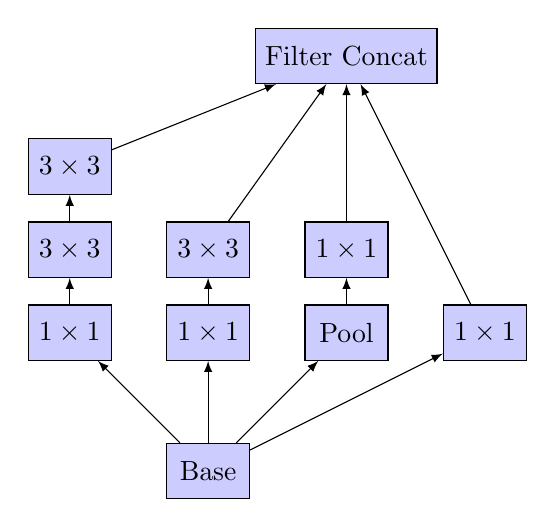
\begin{tikzpicture}[node distance=1.6cm]

    \node (concat) [block] {Filter Concat};

    \node (211) [block, below of=concat, node distance=7em] {$1\times1$};
    \node (233) [block, left of=211] {$3\times3$};
    \node (255) [block, left of=233] {$3\times3$};

    \node (333) [block, above of=255, node distance=3em] {$3\times3$};

    \node (pool) [block, below of=211, node distance=3em] {Pool};

    \node (1111) [block, left of=pool] {$1\times1$};
    \node (1112) [block, left of=1111] {$1\times1$};
    \node (1113) [block, right of=pool] {$1\times1$};

    \node (base) [block, below of=1111] {Base};

    
    \draw[arrow] (base) -- (1111);
    \draw[arrow] (base) -- (1112);
    \draw[arrow] (base) -- (pool);
    \draw[arrow] (base) -- (1113);

    \draw[arrow] (pool) -- (211);
    \draw[arrow] (1111) -- (233);
    \draw[arrow] (1112) -- (255);
    \draw[arrow] (1113) -- (concat);

    \draw[arrow] (255) -- (333);
    \draw[arrow] (333) -- (concat);
    \draw[arrow] (233) -- (concat);
    \draw[arrow] (211) -- (concat);

    

\end{tikzpicture}
    \captionof{figure}{Inception ModuleV2}
    \label{fig:incept_modul2}
\end{minipage}




\subsubsection{Mobilenet}


Das MobileNet \cite{howardMobileNetsEfficientConvolutional2017a}
wurde mit dem Ziel egschaffen, durch geringere 
komplexität, für Mobile Endgeräte oder Embedded Anwendungen 
geeignet zu sein.

Dafür wurden die üblichen \textit{full convolutional Layer}
mit sogenannten \textit{Depthwise Seperable 
Convolutions} ersetzt, welche die Faltung in zwei seperaten 
Layern ausführt. Zuerst wird eine \textit{Depthwise  
Convolutions} auf die drei Farbchannel getrennt ausgeführt.
Anschleißend führt eine \textit{pointwise convolution}
mit $1\times1$ Filter dise wieder zusammen.



In der zweiten version des MobileNet
\cite{sandlerMobileNetV2InvertedResiduals2019},
wurden, die \textit{Depth-wise Separable Convolutions}
wie folgt abgeändert:

Zuerst wird eine $1\times1$ Convolution mit ReLU
Aktivierungsfunktion ausgefühtr, anschließend die 
\textit{Depthwise Convolutions}, gefolgt 
von einer weiteren $1\times1$ mit linearer 
Aktivierungsfunktion.


Desweiteren soll wie beim \textit{ResNet} eine 
\textit{residual connection}, welche Ein- mit Ausgabe 
eines Blocks verbindet, 
den Gradientenfluss unterstützen, wie in Abbildung 
\ref{fig:mobilenetv2} dargestellt ist.
%bild: https://towardsdatascience.com/mobilenetv2-inverted-residuals-and-linear-bottlenecks-8a4362f4ffd5
\begin{figure}[H]
    \centering
    \includegraphics[width=0.5\textwidth]{mobilenet_v2.png}
    \caption{MobilenetV2}
    \label{fig:mobilenetv2}
\end{figure}


%---------------- SUBSECTION: Obj Detection ----------------
\subsection{Objekterkennung}\label{subsec:objdet_det}

Neben der Information, was sich auf einem Bild befindet geht 
es bei der Objekt Erkennung auch darum herausfinden wo sich das 
Objekt auf dem Bild befindet.
Dafür wird die CNN Architektur so erweitert, dass dem 
Modell neben den Klassenlabels auch die Koordinaten 
der Bounding Boxen für das training mit übergeben werden.
Bounding Boxen umrahmen wie in Abbildung 
\ref{fig:class_vs_det} das Objekt auf dem Bild und 
werden meist über Regressionsverfahren 
angenähert.

Das gesammt Framework zur Objekterkennung 
verwendet dabei ein Basis CNN z.B. eines der in 
\ref{subsubsec:architectures} dargestellen. 

Das finden von Regionen, welche Objekte enthalten, 
kann dabei in einem seperaten, Netzwerk, welches 
Selective Search oder Vorschlagsgenerierer 
verwendet, stattfinden.



\vspace{1cm}
\begin{minipage}{0.5\textwidth}
    \centering
    Classification
\end{minipage}
\begin{minipage}{0.5\textwidth}
    \centering
    Detection
\end{minipage}
\begin{figure}[H]
    \centering
    \includegraphics[width=0.8\textwidth]{classification_detection.jpeg}
    \caption{Unterschied: Classification - Detection}
    \label{fig:class_vs_det}
\end{figure}




%------------------- SECTION: Hardware ----------------------
\section{Neural Compute Stick 2}\label{ncs2}

Da das Training und die Inferenz von Deep Learning Algorithmen
sehr rechenintensiv ist, werden entsprechen leistungsfähige 
Prozessoren benötigt. Dabei ist die Ausführung auf einer GPU 
(Graphical Processor Unit) meist effizienter als auf einer 
CPU (Central Processor Unit).

Anwendungen die auf eingebetteten Systemen laufen, wie etwa 
auf einem Raspberry Pi, kommen dabei schnell an ihre 
Grenzen.

Eine möglichkeit ist es die Bilddaten für die 
Verrechnung an eine Cloud zu senden, wo sie 
von einem leistungsstärkeren Rechner inferiert und 
dann wieder zurückgesendet werden.

Sollen die Daten, wie es beim Edge Computing der Fall ist, 
auf dem Anwendungsgerät direkt verarbeitet werden,
gibt es speziell für die Inferenz von Deep Learing Algorithmen
geeignete Hardware.
Durch Fokus auf paralletlität anstatt Taktrate können 
für Neuronale Netze spezifische Rechenoperationen 
wie z.B. die Matrixmultiplikation besonders effizient 
durchgeführt werden.

Die Inferenzbeschleunigende Hardware kann dabei entweder
als eigenständiges \textit{System on Chip (SoC)}
System wie z.B. der \textit{Nvidia Jetson TX2} agieren, oder
in verbindung mit einem Host Pc, wie der, in der Arbeit 
verwendeten, Neural Compute Stick 2 (NCS2).

Der in \ref{fig:ncs2} abgebildete NCS2 verwendet 
für die Inferenz eine Movidius Myriad X Vision Processing Unit (VPU),
welche in Abbildung \ref{fig:myriad} dargestellt ist.

Diese besteht wie in der Masterarbeit
\cite{haussermannFunktionUndEffizienz}
nachzulesen ist, aus der Neural Compute Engine 
zur beschleunigten berechnung Neuronaler Netze, einem
Bildbeschleuniger, 16 SHAVE Prozessoren, einem 
Bildsignalprozessor sowie einem RISC CPU Core.

\vspace{1cm}
\begin{minipage}{0.4\textwidth}
    \centering
    \includegraphics[width=\textwidth]{ncs2_top.jpg}
    \captionof{figure}{NCS2}
    \label{fig:ncs2}
\end{minipage}
\begin{minipage}{0.6\textwidth}
    \centering
    \includegraphics[width=\textwidth]{myriad.png}
    \captionof{figure}{Myriad Chip}
    \label{fig:myriad}
\end{minipage}


\subsection{OpenVino Toolkit}

Um die Inferenz eines trainierten Deep Learing Modells auf dem
Neural Compute Stick auszuführen, wird das Toolkit 
\textit{OpenVino} verwendet.
Dieses ist eine Plattform zur Otimierung und Inferenz von 
CNN basierten Modellen auf verschiedener Intel Hardware.

Dabei wird ein eigenes Dateiformat verwendet, die \textit{Intermediate 
Representation} (IR), welche die Struktur des Modells 
in einer Xml-Datei (.xml) und die trainierten Gewichte in 
einer Binary Datei (.bin) abbildet.
Mit dem \textit{Model Optimizer} können Modelle welche in den 
den Frameworks TensorFlow, Caffe, ONNX, Kaldi, oder MXNET 
trainiert wurden, in das IR Format konvertiert werden.

Um diese dann auf die entsprechende Hardware zu laden und anwendbar 
zu machen, wird die auch in OpenVino enthaltene
\textit{InferenceEngine} verwendet.
Diese bietet eine Api mit der aus der Anwendung heraus in den 
Programmiersprachen C++ oder Python auf die Funktionen der 
InferenceEngine zugegriffen werden können.

In Abbildung \ref{fig:openvinoflow} ist der Workflow mit 
Openvino, welcher das Training eines Deep Learning Modells 
mit der Implementierung einer Nutzer Anwendung verbindet, 
dargestellt.


\vspace{1cm}
\begin{figure}[H]
    \centering
    \def\svgwidth{0.8\textwidth}
    \input{Bilder/open_vino_workflow_neu.pdf_tex}
    \caption{OpenVino Workflow}
    \label{fig:openvinoflow}
\end{figure}
